\documentclass[conference]{IEEEtran}
\IEEEoverridecommandlockouts
\usepackage{cite}
\usepackage{amsmath,amssymb,amsfonts,amsthm}
\usepackage{graphicx}
\usepackage{textcomp}
\usepackage{xcolor}
\usepackage{booktabs}
\usepackage{tikz}
\usetikzlibrary{shapes.geometric, arrows.meta, shadows}
\usepackage[caption=false,font=footnotesize]{subfig}
\usepackage{hyperref}
\hypersetup{colorlinks=true, linkcolor=blue, citecolor=blue, urlcolor=blue}

\graphicspath{{../../src/figures/}}
\newtheorem{proposition}{Proposition}
\setlength{\columnsep}{0.22in}

\begin{document}

\title{A Certified Admission Gate for Online Reconfiguration of Time-Sensitive Networks}

%Trang's work [Updated]: Authors and affiliations (IBISC, Univ. Evry; CEDRIC, Cnam). ORCID of S. Bouzefrane checked in the ORCID registry.
\author{\IEEEauthorblockN{Huyen-Trang Le{\href{https://orcid.org/0009-0004-3738-0235}{
\includegraphics[scale=0.13]{ORCIDiD_icon64x64.png}}}}
\IEEEauthorblockA{\textit{IBISC Laboratory} \\
\textit{Universit\'e d'\'Evry Paris-Saclay}\\
\'Evry-Courcouronnes, France \\
huyen.le@etud.univ-evry.fr}
\and
\IEEEauthorblockN{Samia Bouzefrane{\href{https://orcid.org/0000-0002-0979-1289}{
\includegraphics[scale=0.13]{ORCIDiD_icon64x64.png}}}}
\IEEEauthorblockA{\textit{CEDRIC Laboratory} \\
\textit{Conservatoire National des Arts et M\'etiers (Cnam)}\\
Paris, France \\
samia.bouzefrane@lecnam.net}
}

\maketitle

%Trang's work [Updated]: Abstract summarising problem, gate and measured results.
\begin{abstract}
Time-Sensitive Networking (TSN) guarantees worst-case latency only for a configuration that has been fixed and verified offline. When flows join a running network, fast optimisers (heuristics, ILP/SMT solvers, learned policies) can propose new configurations, but none of them certifies that every deadline still holds. We place a \emph{certified admission gate} between any such proposer and the network. The gate accepts a flow only together with a certificate: a per-hop witness of the network-calculus bound of every affected flow, which an independent checker of about fifty lines re-verifies without trusting the analysis code. We model 1\,Gbit/s switches with non-preemptive static priority and token-bucket flows, and bound delays with Total Flow Analysis. An incremental variant of the gate recomputes only the ports a request can affect and yields bit-identical bounds. On line and tree topologies with 1,000 seeded requests and 10 seeds, our bounds match the reference tool panco to a relative difference of $3.3\times10^{-16}$ per hop and $2.9\times10^{-6}$ end to end, no simulated delay exceeds its bound across 2,118 admitted flows, and the incremental gate is $1.9$--$2.0\times$ faster than full recomputation. All code, data and figures are reproducible from a public repository.
\end{abstract}

\begin{IEEEkeywords}
Time-Sensitive Networking, network calculus, admission control, certification, worst-case delay
\end{IEEEkeywords}

% ---------------------------------------------------------------------------
%Trang's work [Updated]: More contextual text before jumping into technology.
\section{Problem}
\label{sec:problem}

Factories, vehicles and aircraft increasingly replace dedicated fieldbuses with a single Ethernet network shared by control loops, sensors, video and best-effort traffic. For control traffic, a message that arrives late is not a slower service but a failure: a robot arm or a braking system acts on stale data. What these systems need from the network is therefore not a good average latency but a \emph{guaranteed worst case}, and that guarantee must survive while the system evolves, as machines, sensors and applications are added during operation.

Time-Sensitive Networking (TSN), a set of IEEE 802.1Q mechanisms~\cite{ieee8021q}, provides such bounded latency on switched Ethernet. Its guarantees rest on an analysis of the whole flow set: a worst-case delay bound computed with network calculus~\cite{cruz1991calculus,leboudec2001nc} or a schedule synthesised offline~\cite{xue2024tsn}. Real deployments, however, are not static. Flows are added while the network runs, and every change can increase the delay of flows already admitted, including flows on other paths whose traffic shares a port.

Many tools can \emph{propose} a change quickly: greedy heuristics, ILP or SMT schedulers~\cite{xue2024tsn}, and, increasingly, deep reinforcement learning policies. Their outputs are optimised, not proven. A learned policy in particular gives no worst-case guarantee, and even an exact solver is only as trustworthy as its encoding and implementation. For safety-critical traffic, the question at reconfiguration time is binary and must be answered with evidence: \emph{after this change, does every admitted flow still meet its deadline?}

We answer it with an \emph{admission gate}, placed between any proposer and the network, in the spirit of a safety shield for learned controllers~\cite{alshiekh2018shield}. The gate receives one request at a time and returns a verdict together with a \emph{certificate}. A change is committed only if the certificate passes an independent checker. Fig.~\ref{fig:architecture} shows the setting and the pipeline. The guarantee is a safety property relative to the network model: it holds as far as the model of Section~\ref{sec:model} describes the real network.

\textbf{Contributions.} (i) A gate $\mathrm{admit}(S, f) \to (\mathit{verdict}, \mathit{certificate})$ for non-preemptive static-priority TSN, whose certificates are checked by a small, separate checker with an explicit soundness argument (Section~\ref{sec:gate}). (ii) An incremental gate that recomputes only the ports a request can affect and provably returns the same bounds as full recomputation. (iii) A validation against the reference tool panco~\cite{bouillard2022panco}, a packet-level simulator and unit tests, with all results reproducible (Section~\ref{sec:results}). (iv) An explicit list of what the guarantee does not cover (Section~\ref{sec:limits}).

%Trang's work [Updated]: Architecture figure redrawn across both columns: (a) TSN topology in the style of Zhao et al. Fig. 1, (b) packet handling by priority at an NP-SP output port, (c) admission gate pipeline. Colours match the result figures: red = class 0, green = class 1.
\definecolor{cHigh}{HTML}{D62728}
\definecolor{cLow}{HTML}{2CA02C}
\definecolor{cReq}{HTML}{1F77B4}
\definecolor{cNode}{HTML}{EEF3FA}
\definecolor{cSwitch}{HTML}{E8E8E8}
\tikzset{
  every picture/.append style={font=\scriptsize, >=Latex},
  es/.style={ellipse, draw=black!70, fill=cNode, minimum width=0.8cm, minimum height=0.4cm, inner sep=0pt, drop shadow={opacity=0.2}},
  sw/.style={rectangle, rounded corners=3pt, draw=black!70, fill=cSwitch, minimum width=0.85cm, minimum height=0.42cm, drop shadow={opacity=0.2}},
  link/.style={{Latex[length=1.5mm]}-{Latex[length=1.5mm]}, thick, black!75},
  route/.style={-{Latex[length=2mm]}, thick, rounded corners=5pt},
  pkt/.style={draw=black!70, line width=0.3pt, minimum height=0.3cm, inner sep=0pt},
  flow/.style={-{Stealth[length=1.9mm, width=1.6mm]}, line width=0.8pt, line cap=round, shorten <=1.5pt, shorten >=1pt},
  box/.style={rectangle, rounded corners=3pt, draw=black!70, align=center, minimum height=0.55cm, drop shadow={opacity=0.2}},
  data/.style={rectangle, rounded corners=2pt, draw=black!60, dashed, align=center, fill=white, minimum height=0.55cm},
}
\begin{figure*}[t]
\centering
% ---------------- (a) TSN network topology example ----------------
\subfloat[TSN topology]{%
\begin{tikzpicture}
  \node[es] (es1) at (0, 1.9) {ES$_1$};
  \node[es] (es2) at (0, 0.5) {ES$_2$};
  \node[sw] (sw1) at (1.6, 1.2) {SW$_1$};
  \node[sw] (sw2) at (3.7, 1.2) {SW$_2$};
  \node[es] (es3) at (5.3, 1.9) {ES$_3$};
  \node[es] (es4) at (5.3, 0.5) {ES$_4$};
  \node[sw] (sw3) at (2.65, -0.1) {SW$_3$};
  \foreach \a/\b in {es1/sw1, es2/sw1, sw1/sw2, sw2/es3, sw2/es4, sw1/sw3, sw2/sw3}
    \draw[link] (\a) -- (\b);
  \draw[route, cHigh, dashed] (0.4, 2.2) -- (1.6, 1.74) -- (3.7, 1.74) -- (4.9, 2.2);
  \draw[route, cReq, densely dotted, very thick] (0.4, 0.78) -- (1.6, 1.56) -- (3.7, 1.56) -- (4.88, 1.82);
  \draw[route, cLow, dashed] (0.4, 0.2) -- (1.6, 0.7) -- (3.7, 0.7) -- (4.9, 0.2);
  \node[cHigh] at (0.9, 2.22) {$f_1$};
  \node[cReq]  at (0.3, 1.2) {$f$};
  \node[cLow]  at (0.9, 0.18) {$f_2$};
  \node[font=\scriptsize\itshape] at (2.65, 1.0) {port $p$};
\end{tikzpicture}}%
\hfil
% ---------------- (b) packet handling at an NP-SP output port ----------------
\subfloat[NP-SP output port $p$]{%
\begin{tikzpicture}
  % arrivals
  \node[pkt, fill=cHigh, minimum width=0.15cm] (a1) at (0.12, 2.05) {};
  \node[pkt, fill=cReq,  minimum width=0.15cm] (a2) at (0.12, 1.25) {};
  \node[pkt, fill=cLow,  minimum width=0.34cm] (a3) at (0.2, 0.45) {};
  \foreach \n/\y/\c in {a1/2.05/cHigh, a2/1.25/cReq, a3/0.45/cLow} \draw[flow, \c] (\n.east) -- (0.88, \y);
  \node[cHigh] at (0.12, 2.36) {$f_1$};
  \node[cReq]  at (0.12, 1.56) {$f$};
  \node[cLow]  at (0.2, 0.76) {$f_2$};
  % classifier
  \node[rectangle, rounded corners=2pt, draw=black!70, fill=cSwitch, minimum width=0.4cm, minimum height=2.2cm, drop shadow={opacity=0.2}] at (1.08, 1.25) {};
  \node[rotate=90] at (1.08, 1.25) {classify by $k$};
  % FIFO queues (open on the left)
  \foreach \y/\lab/\c in {1.8/class 0 (high)/cHigh, 0.7/class 1 (low)/cLow} {
    \draw[thick, black!75] (1.72, \y+0.24) -- (2.95, \y+0.24) -- (2.95, \y-0.24) -- (1.72, \y-0.24);
    \node[anchor=south west, inner sep=1pt] at (1.72, \y+0.25) {\lab};
    \draw[flow, \c] (1.28, \y) -- (1.84, \y);
  }
  \node[pkt, fill=cHigh, minimum width=0.15cm] at (2.81, 1.8) {};
  \node[pkt, fill=cReq,  minimum width=0.15cm] at (2.61, 1.8) {};
  \node[pkt, fill=cHigh, minimum width=0.15cm] at (2.41, 1.8) {};
  \node[pkt, fill=cLow,  minimum width=0.34cm] at (2.72, 0.7) {};
  \node[pkt, fill=cLow,  minimum width=0.34cm] at (2.32, 0.7) {};
  % strict-priority selector and link
  \node[circle, draw=black!70, fill=white, minimum size=0.52cm, inner sep=0pt, drop shadow={opacity=0.2}] (sp) at (3.5, 1.25) {SP};
  \draw[flow, cHigh] (2.95, 1.8) to[out=0, in=125] (sp);
  \draw[flow, cLow]  (2.95, 0.7) to[out=0, in=235] (sp);
  \node[cHigh, font=\tiny] at (3.5, 1.92) {1st};
  \node[cLow,  font=\tiny] at (3.5, 0.58) {2nd};
  \draw[flow, black!75, line width=1.1pt] (sp.east) -- (5.1, 1.25) node[below left, inner sep=2pt] {$C$};
  \node[pkt, fill=cLow, minimum width=0.34cm] at (4.3, 1.25) {};
  \node[align=center, font=\tiny] at (4.3, 1.72) {in transmission,\\not preempted};
  \node[align=center, font=\tiny] at (4.25, 0.5) {class 0 waits\\at most $L_{lo}/C$};
\end{tikzpicture}}%
\hfil
% ---------------- (c) admission gate functionality ----------------
\subfloat[Admission gate]{%
\begin{tikzpicture}
  \node[box, minimum width=2.2cm, fill=white] (prop) at (1.9, 3.0) {Proposer\\(heuristic, ILP, DRL)};
  \node[box, minimum width=2.2cm, fill=cReq!12] (gate) at (1.9, 1.85) {Admission gate\\TFA \eqref{eq:hop}--\eqref{eq:e2e}};
  \node[box, minimum width=2.2cm, fill=cLow!15] (chk) at (1.9, 0.75) {Checker C0--C6};
  \node[box, minimum width=2.2cm, fill=white] (com) at (1.9, -0.2) {commit $S \cup \{f\}$};
  \node[data, minimum width=0.8cm] (st) at (0.05, 1.85) {$S$};
  \node[data, minimum width=0.8cm] (db) at (3.95, 0.75) {flow\\DB};
  \draw[->, thick] (prop) -- node[right, pos=0.45] {request $f$} (gate);
  \draw[->, thick] (gate) -- node[right, pos=0.45] {certificate} (chk);
  \draw[->, thick] (chk) -- node[right, pos=0.45] {pass} (com);
  \draw[->] (st) -- (gate);
  \draw[->] (db) -- (chk);
  \draw[->, black!60] (com.west) -| (st.south);
  \draw[->, dashed, cHigh] (gate.east) -- ++(0.55, 0) |- node[right, pos=0.25] {reject} (prop.east);
\end{tikzpicture}}
\caption{System architecture. (a)~Admitted flows $f_1$ (class 0) and $f_2$ (class 1) and a new class-0 request $f$ share output port $p$. (b)~At $p$, frames are classified by priority into FIFO queues; the strict-priority (SP) selector serves class 0 first but cannot preempt a class-1 frame already in transmission, which is the $L_{lo}$ term of~\eqref{eq:hop}. (c)~A proposed change is committed only if the gate's certificate passes the independent checker, which also reads the flow database (C0); a rejection returns the violated flows to the proposer.}
\label{fig:architecture}
\end{figure*}


% ---------------------------------------------------------------------------
%Trang's work [Updated]: System model and the NP-SP per-hop, burst and end-to-end bounds (TFA).
\section{Model}
\label{sec:model}

\textbf{Network.} The network is a set of switches and end stations joined by full-duplex links of rate $C = 1$\,Gbit/s. Each direction of a link is an output \emph{port}, served by the transmitting node. A switch adds a constant processing delay $t_{\mathit{proc}}$. Routing is fixed: each source--destination pair uses one shortest path, and end stations do not forward. When the network is built, we compute the dependency graph between ports induced by all possible routes and require it to be acyclic (\emph{feed-forward}); its topological order is reused for every flow set.

\textbf{Flows.} A flow $f$ has a source, a destination, a token-bucket arrival curve $\alpha_f(t) = b_f + r_f t$ at its source, a maximum frame size $L_f \le b_f$, a priority class $k_f$ (0 is the highest) and an end-to-end deadline $D^{\max}_f$. Ports use non-preemptive static priority (NP-SP), FIFO within a class.

\textbf{Per-hop bound.} Consider class $k$ at a port $p$. Let $B_H, R_H$ be the sums of input bursts and rates of the flows of higher priority at $p$, $B_k, R_k$ the same sums for class $k$, and $L_{lo}$ the largest frame of lower priority. Because transmission is not preempted, one lower-priority frame can block class $k$; the higher classes take at most $B_H + R_H t$. Class $k$ therefore receives the residual rate-latency service curve
\begin{equation}
\beta_k(t) = (C - R_H)\left[t - \frac{B_H + L_{lo}}{C - R_H}\right]^+ ,
\end{equation}
and, as the class aggregate is constrained by $B_k + R_k t$, the delay of any class-$k$ frame at $p$ is bounded by the horizontal deviation~\cite{leboudec2001nc,bouillard2018dnc}
\begin{equation}
d_k = \frac{B_H + L_{lo} + B_k}{C - R_H} + t_{\mathit{proc}}, \quad \text{valid if } R_H + R_k \le C .
\label{eq:hop}
\end{equation}
If the rate condition fails, the port is unstable and $d_k = \infty$.

\textbf{Propagation.} A flow that leaves a server with delay bound $d$ has output arrival curve $\alpha(t + d)$, so its burst at the next hop is
\begin{equation}
b' = b + r_f\, d_k .
\label{eq:burst}
\end{equation}
Total Flow Analysis (TFA) visits ports in topological order, applies~\eqref{eq:hop} with the propagated bursts~\eqref{eq:burst}, and bounds the end-to-end delay of $f$ along its path $\mathcal{P}_f$ by
\begin{equation}
D_f = \sum_{h \in \mathcal{P}_f} d_{k_f}^{(h)} .
\label{eq:e2e}
\end{equation}
A flow set is \emph{schedulable} if every port is stable and $D_f \le D^{\max}_f$ for every flow.

% ---------------------------------------------------------------------------
%Trang's work [Updated]: Gate interface, certificate, checker conditions C0--C6 with soundness sketch, full vs. incremental gate.
\section{The Admission Gate}
\label{sec:gate}

\textbf{Interface and invariant.} The gate holds the admitted set $S$. On a request $f$, it analyses $S \cup \{f\}$ and accepts if and only if that set is schedulable. Invariant: \emph{every flow in $S$ meets its deadline under the model.} A request is rejected not only when $f$ itself would miss its deadline, but also when admitting $f$ would make an already admitted flow miss its own; the rejection lists every violated flow and reason.

\textbf{Certificate.} An acceptance carries, for each flow, a \emph{witness}: its parameters, its path, and for each hop the input burst $b_{in}$, the aggregates $(B_H, R_H, L_{lo}, B_k, R_k)$ and the delay $d$, plus the end-to-end bound. It also carries a fingerprint of the admitted set before and after the request: the XOR of a SHA-256 hash of each flow, which is order-independent and updated in $O(1)$.

\textbf{Checker.} The checker receives the topology, the witnesses and the operator's flow database, and re-verifies seven conditions without calling the analysis code:
\begin{itemize}
\item[C0] there is exactly one witness per admitted flow, with that flow's own parameters;
\item[C1] each witnessed path is the fixed route of the flow;
\item[C2] the first input burst is at least $b_f$;
\item[C3] each next input burst is at least $b_{in} + r_f d$ (Eq.~\eqref{eq:burst});
\item[C4] at each port, the claimed aggregates are at least the sums (or maximum, for $L_{lo}$) recomputed from all witnesses crossing that port;
\item[C5] $R_H < C$, $R_H + R_k \le C$, and $d$ is at least the right-hand side of~\eqref{eq:hop};
\item[C6] the end-to-end bound is at least the sum of hop delays and at most the deadline.
\end{itemize}

\begin{proposition}
If a certificate passes C0--C6, every admitted flow meets its deadline under the model of Section~\ref{sec:model}.
\end{proposition}
\begin{proof}[Proof sketch]
The bound~\eqref{eq:hop} is non-decreasing in $B_H$, $R_H$ (for $R_H < C$), $L_{lo}$ and $B_k$. We show by induction over the topological order of ports that every witnessed input burst over-approximates the true one. At the first hop this is C2. Assume it holds for all flows entering port $p$. By C0 and C1, the witnesses at $p$ are exactly the flows that cross $p$, so by C4 the claimed aggregates over-approximate the true ones; by monotonicity and C5 the claimed $d$ bounds the true delay at $p$. The true output burst is then at most $b_{in} + r_f d$, which by C3 is at most the next witnessed input burst. Feed-forwardness makes the induction well founded. Summing the per-hop bounds, C6 gives a true end-to-end delay at most the claimed bound, which is at most the deadline.
\end{proof}

C0 is needed: omitting a flow from the certificate only lowers the aggregates of the others, so all remaining conditions would still pass. Comparing with the flow database is the only way to detect the omission, and our tests confirm that the checker rejects it only when the database is supplied. The checker is about fifty lines of code, separate from the analysis, and uses a relative tolerance of $10^{-9}$ for floating-point comparisons.

\textbf{Full and incremental gates.} The \emph{full gate} reruns TFA over $S \cup \{f\}$ for every request. The \emph{incremental gate} keeps the per-port results, bursts and bounds of $S$ in a cache. For a request, it pushes the ports of the new path into a priority queue keyed by topological index, re-evaluates each popped port, and enqueues the next port of a flow only if that flow's output burst changed. It writes into overlays, so the cache is untouched until the verdict, and it issues a \emph{delta certificate} that holds witnesses only for flows whose bounds changed. Both gates call the same pure port function, which sums with exactly rounded summation (\texttt{math.fsum}) and is therefore independent of the order of flows. By induction over the topological order, both gates feed it identical inputs at every port, so they return the same verdicts and \emph{bit-identical} bounds, not merely close ones.

% ---------------------------------------------------------------------------
%Trang's work [Updated]: Results from src/results/*.csv; figures rebuilt with src/experiments/plot_figures.py.
\section{Results}
\label{sec:results}

\textbf{Setup.} We use two feed-forward topologies with 48 ports each: a \emph{line} of 5 switches with 4 end stations per switch, and a \emph{tree} with one core switch and 4 edge switches with 5 end stations each; $C = 1$\,Gbit/s and $t_{\mathit{proc}} = 1\,\mu$s. Requests are drawn between random end-station pairs from two classes. Class~0 (control, probability 0.3) has 64--256\,B frames, periods of 0.25--1\,ms and deadlines of 0.1--0.5\,ms. Class~1 (stream) has 500--1500\,B frames, bursts of one or two frames, periods of 0.125--1\,ms and deadlines of 0.5--2\,ms. Each run submits 1,000 requests in sequence; we use 10 seeds per topology and run both gates on the same sequence. The code is single-threaded CPython 3.14.

\begin{figure}[t]
\centering
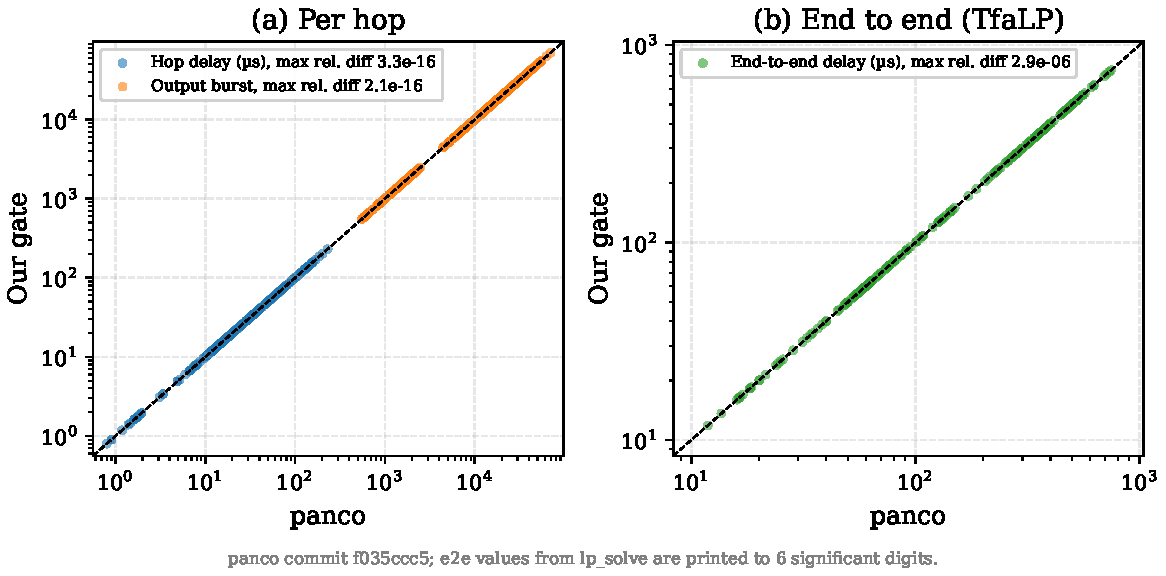
\includegraphics[width=\columnwidth]{panco_agreement.pdf}
\caption{Bounds of our gate against panco~\cite{bouillard2022panco}, per hop (837 values) and end to end (210 values, TfaLP).}
\label{fig:panco}
\end{figure}

\textbf{Agreement with panco.} We compare our analysis with panco~\cite{bouillard2022panco} on five scenarios: a hand-computed two-flow example and two seeds of 60 requests on each topology, with $t_{\mathit{proc}} = 0$. Per hop, panco's static-priority residual server gives the delay and output burst that we compare with~\eqref{eq:hop} and~\eqref{eq:burst}. End to end, panco builds one FIFO network per class from residual servers and solves TFA as a linear program, independently of our propagation code. The 290 hop delays and 547 output bursts agree to a relative difference of at most $3.3 \times 10^{-16}$, that is, to floating-point precision; the 210 end-to-end bounds agree to $2.9 \times 10^{-6}$, the precision at which lp\_solve prints its results (Fig.~\ref{fig:panco}).

\begin{figure}[t]
\centering
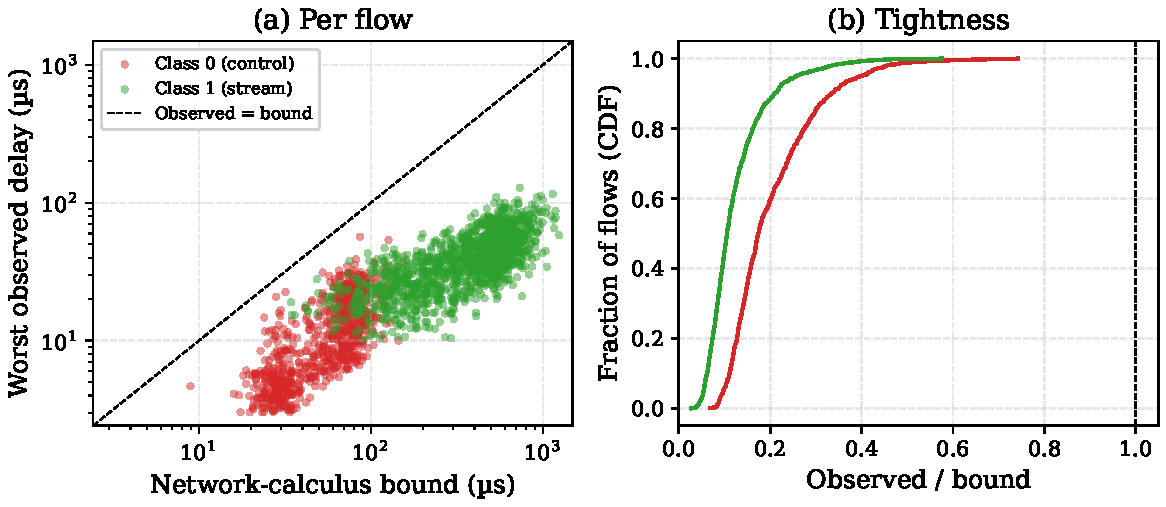
\includegraphics[width=\columnwidth]{bound_tightness.pdf}
\caption{Worst simulated delay against the bound for 2,118 admitted flows (10\,ms simulated, line and tree, 10 seeds). (a)~Per flow; (b)~CDF of observed/bound.}
\label{fig:sim}
\end{figure}

\textbf{Simulation.} A discrete-event, packet-level simulator replays every admitted set: each flow emits its burst at a random offset and then frames at rate $r_f$, and ports serve NP-SP queues frame by frame. Over 2,118 admitted flows, no observed delay exceeds its bound (Fig.~\ref{fig:sim}). The median ratio of observed delay to bound is 0.17 for control traffic and 0.11 for stream traffic, with maxima of 0.74 and 0.58. These ratios are a sanity check, not a measure of tightness: the simulator does not search for the worst-case alignment of bursts.

\begin{figure}[t]
\centering
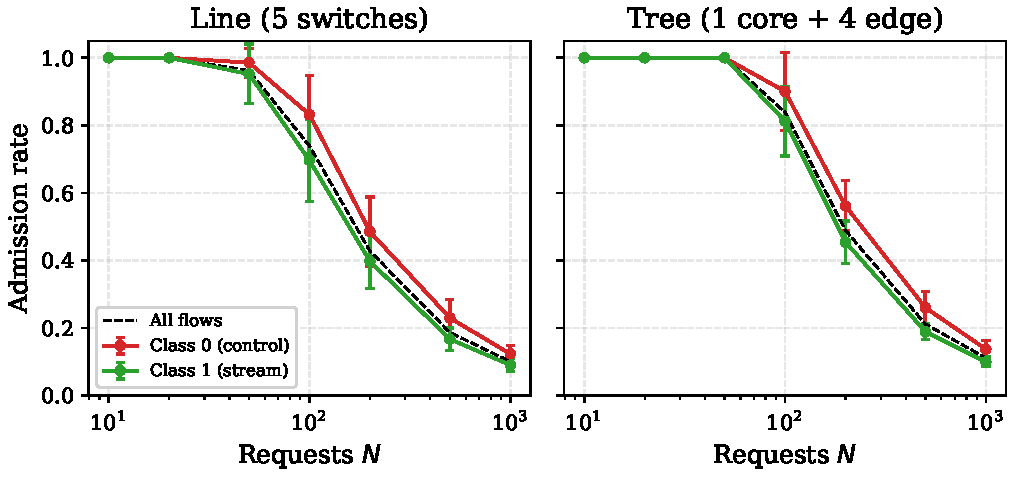
\includegraphics[width=\columnwidth]{admission_rate.pdf}
\caption{Fraction of the first $N$ requests accepted, per class (mean $\pm$ std over 10 seeds).}
\label{fig:rate}
\end{figure}

\textbf{Admission rate.} Both networks accept every request up to about 50, then saturate (Fig.~\ref{fig:rate}). After 1,000 requests, $100 \pm 20$ flows are admitted on the line and $111 \pm 16$ on the tree, an overall rate of 10--11\,\%. Control traffic is accepted slightly more often than stream traffic, because its higher priority shields it from most interference, but its tight deadlines still cause rejections once higher-priority bursts accumulate.

\begin{figure}[t]
\centering
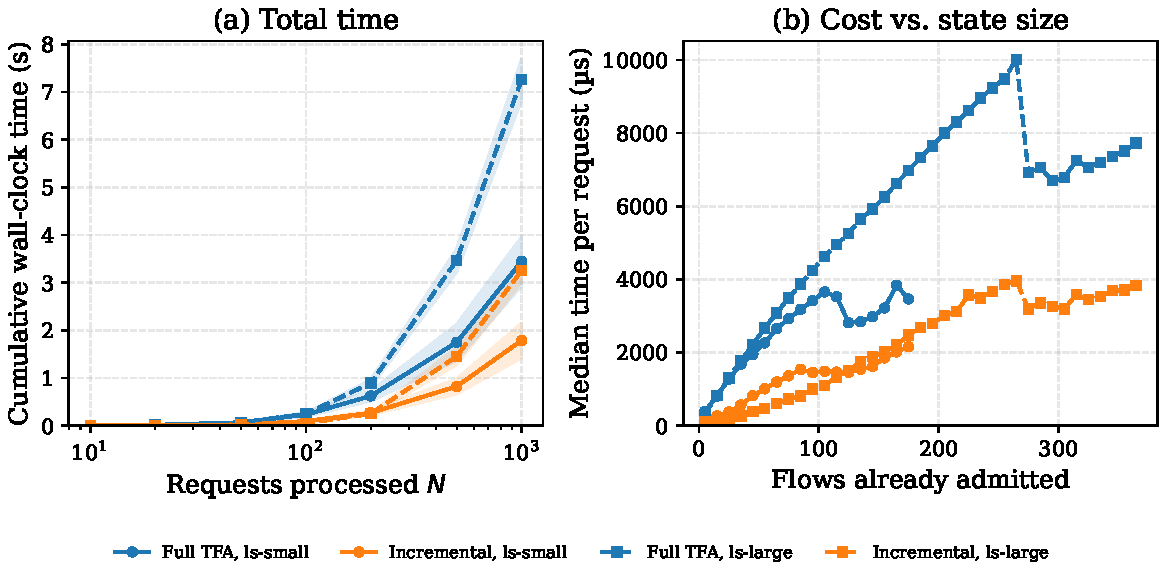
\includegraphics[width=\columnwidth]{scalability.pdf}
\caption{Run time of the full and incremental gates. (a)~Cumulative time over $N$ requests; (b)~median time per request against the number of admitted flows.}
\label{fig:time}
\end{figure}

\begin{table}[t]
\centering
\caption{Admission time per request ($\mu$s), 10 seeds $\times$ 1,000 requests.}
\label{tab:time}
\begin{tabular}{llrrr}
\toprule
Topology & Gate & Median & p95 & Speed-up \\
\midrule
Line & Full        & 1944 & 2745 & \\
     & Incremental &  964 & 1587 & $2.02 \pm 0.13$ \\
Tree & Full        & 2202 & 3718 & \\
     & Incremental & 1186 & 1750 & $1.91 \pm 0.23$ \\
\bottomrule
\end{tabular}
\end{table}

\textbf{Run time.} Over all runs, the full and incremental gates return identical verdicts, and the final bounds of both are equal bit for bit. The incremental gate is $2.02\times$ faster on the line and $1.91\times$ on the tree over 1,000 requests (Table~\ref{tab:time}), and its cost per request grows more slowly with the number of admitted flows (Fig.~\ref{fig:time}b). The gain is modest because these networks are small: a request still re-evaluates a median of 19 of the 48 ports. A median decision takes about 1\,ms in Python.

\textbf{Tests.} Eighteen unit tests cover a hand-computed example that the gate reproduces to a relative $10^{-12}$, equality of the two gates on random workloads, the simulator, and tampered certificates: halving one hop delay is rejected by C5, and omitting a flow is rejected by C0 only.

% ---------------------------------------------------------------------------
%Trang's work [Updated]: Limitations of the model, the analysis, the certification and the evaluation.
\section{Limitations}
\label{sec:limits}

\textbf{Model.} The guarantee is only as good as the model. We assume a single link rate, fixed shortest-path routing, feed-forward port dependencies and strict NP-SP. Credit-based and time-aware shapers, frame preemption, redundancy and clock effects are not modelled, and Ethernet overheads (preamble, inter-frame gap) must be folded into $L_f$, $b_f$ and $r_f$ by the operator. The processing delay is a constant upper bound.

\textbf{Analysis.} TFA bounds each port separately and propagates bursts hop by hop. It is sound but pessimistic compared with methods that exploit the pay-burst-only-once effect, such as PMOO or LP-based analyses~\cite{bondorf2014discodnc,bouillard2018dnc}. Pessimism lowers the admission rate; it never admits an unsafe flow.

\textbf{Certification.} The soundness argument is a proof sketch on paper, not a mechanised proof, and the checker compares floating-point values with a relative tolerance of $10^{-9}$, which the argument does not account for. The checker is small but not itself verified; a formally verified checker, or exact rational arithmetic, would close both gaps. The certificate attests to the model, not to the configuration actually deployed on the switches.

\textbf{Scope of the evaluation.} The gate only handles new flows; removing a flow and reconfiguring several flows at once are not implemented. The networks are small, saturate at about 100 flows, and only two classes are used, so the measured speed-up of the incremental gate may not carry over to larger networks. The simulator does not reach the worst case, and the run times are those of single-threaded Python on one machine. Finally, no proposer is connected yet: the gate has been tested on random requests only, not behind a heuristic or a learned policy.

% ---------------------------------------------------------------------------
%Trang's work [Updated]: Conclusion and future work aligned with the thesis.
\section{Conclusion}

\textbf{Contribution.} This work makes online traffic allocation in TSN safe to automate. Each time a flow asks for a share of the network, the gate decides whether the ports on its path can still absorb its burst and rate without any admitted flow missing its deadline, and allocates the resources only if they can. Every allocation comes with a certificate that a fifty-line checker re-verifies (C0--C6), so a proposer, even a learned one, can never commit an unsafe allocation under the model. The incremental gate makes this decision in about 1\,ms with bounds bit-identical to full recomputation, and the bounds match panco to numerical precision and hold for all 2,118 simulated flows.

\textbf{Future directions.} Four directions follow. (i)~\emph{Capacity:} TFA is pessimistic and caps admission at about 100 flows on our topologies; tighter analyses that keep checkable certificates would let the same network carry more traffic. (ii)~\emph{Coverage:} credit-based and time-aware shapers and frame preemption must be modelled to allocate traffic in real TSN deployments. (iii)~\emph{Trust:} a mechanised soundness proof and an exact-arithmetic checker would remove the remaining gaps in the guarantee. (iv)~\emph{Allocation policy:} supporting flow removal and batched changes, then placing the gate as a shield behind heuristic, ILP and DRL proposers, will show how much admission capacity certification costs each of them.


\bibliographystyle{IEEEtran}
\bibliography{tsn-references}

\end{document}
